\paragraph{Цель работы:} Ознакомиться с интерфейсом симулятора.

\subsection*{Выполнение}

\begin{enumerate}
	\item Загрузка готового производственного участка с роботом RV-2AJ для изучения интерфейса программного обеспечения.
	\item Изучение окон программной оболочки, панелей инструментов и горячих клавиш.
	\item Экспериментирование с примитивами и свойствами объектов.
	\item Добавление точек захвата к заготовке.
	\item Просмотр примера программы на MELFA-BASIC IV/V.
\end{enumerate}

\begin{figure}[ht]
\centering
	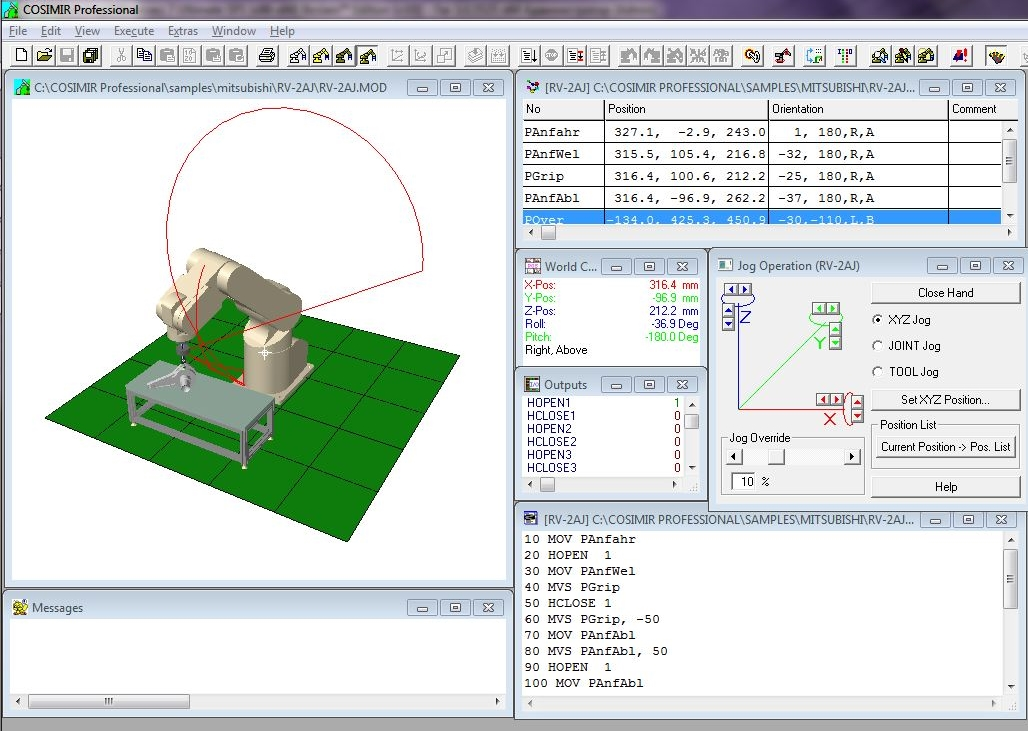
\includegraphics[scale=0.6]{1.png}
	\caption{Результат выполнения работы}
\end{figure}

\subsection*{Выводы}

Программный пакет ``COSIMIR Professional'' служит для симуляции промышленных роботов и моделирования производственных участков, состоящих из робота и деталей, с которыми необходимо провести определенные операции. В этой лабораторной работе мы загрузили готовый производственный участок и познакомились с интерфейсом ПО, а так же поигрались с параметрами объектов и промышленного робота. В процессе изучения работы была также разобрана программа на языке программирования MELFA-BASIC IV/V, использующемся в ПО.

\clearpage